\documentclass[11pt]{article}
\usepackage[margin=0.8in]{geometry}\usepackage{amsmath,graphicx}\pagestyle{empty}
\setlength{\parskip}{4pt}\setlength{\parindent}{0pt}
\begin{document}
{\Large\bf Supernova-type shell wrinkling applied to the CoE setup}\\[2pt]
Expanding $H_0=70$ run: point mass $M$ at the CoE, shells start with $v=k\,r$, $k=160$ km\,s$^{-1}$Mpc$^{-1}$, run time $T=7.86$ Gyr, observer at $D=3.2$ Gpc, view to 787 Mpc. $1\times = 6.08\times10^{51}$ kg (original geometry: $D=58.2$ Gpc, shell $R=14.3$ Gpc, $1\times=7.5\times10^{52}$ kg; same dimensionless run, so all lengths below scale by $58.2/3.2=18.2$).

\section*{1. Shell motion and effective gravity}
\[ \frac{d^2r}{dt^2} = -\frac{G M}{r^2}, \qquad r(0)=r_0,\quad \dot r(0)=k\,r_0, \qquad r(T)=D \]
\[ g_{\rm eff}(t) = -\frac{d^2 r}{dt^2} = \frac{G M}{r(t)^2} \]
$r(t)$: radius of our shell from the CoE; $r_0$: its start radius; $G$: gravitational constant; $g_{\rm eff}$: deceleration felt in the shell frame (points outward, so the dense shell sits ``on top'').

\section*{2. Rayleigh--Taylor growth}
\[ \sigma(t) = \sqrt{A\,k_\lambda(t)\,g_{\rm eff}(t)}, \qquad A=\frac{\rho_{\rm shell}-\rho_{\rm in}}{\rho_{\rm shell}+\rho_{\rm in}}\approx 1, \qquad k_\lambda(t)=\frac{2\pi}{\lambda}\,\frac{D}{r(t)} \]
\[ N(\lambda) = \int_0^T \sigma(t)\,dt \qquad\text{(e-folds; amplitude grows by } e^{N}) \]
$\sigma$: growth rate; $A$: Atwood number; $\rho_{\rm shell},\rho_{\rm in}$: shell and interior densities; $\lambda$: wavelength measured today; $k_\lambda$: physical wavenumber of a ripple that keeps a fixed angle on the stretching shell.

\section*{3. Vishniac thin-shell mode}
\[ \lambda_{\rm V} \approx (2\text{--}5)\,\Delta, \qquad \ell = \frac{2\pi R}{\lambda_{\rm V}}, \qquad \text{needs } \frac{\rho_{\rm shell}}{\rho_0}\gtrsim 10,\ \gamma\to1 \]
$\Delta$: shell thickness; $R$: shell radius; $\ell$: angular mode number; $\rho_0$: density ahead of the shell; $\gamma$: adiabatic index. No shell thickness is defined in our earlier work, so $\Delta/R=0.01$--$0.2$ is scanned (Bertschinger 1983 cosmological blast shells: $\Delta\approx0.03\,r_s$).

\section*{4. Key numbers}
\begin{tabular}{lccc}\hline
 & $1\times$ & $4\times$ & $10\times$\\\hline
start radius $r_0$ (Gpc) & 1.45 & 1.57 & 1.76\\
$g_{\rm eff}$ start / now ($10^{-11}$ m\,s$^{-2}$) & 20 / 4.2 & 69 / 17 & 138 / 42\\
shell speed now (km/s) & 209{,}000 & 171{,}000 & 110{,}000\\
e-folds $N$ at 40 / 100 / 150 Mpc & 6.3 / 4.0 / 3.3 & 12 / 7.4 / 6.0 & 17 / 10.5 / 8.5\\
e-folds at 1000 Mpc & 1.3 & 2.3 & 3.3\\
wavelength with $N=3$ (Mpc) & 180 & 610 & 1200\\\hline
\end{tabular}

Vishniac spacing ($\lambda\approx3\Delta$) on the shell at $D=3.2$ Gpc: $\Delta/R=0.01\to96$ Mpc ($\ell\approx210$), $0.03\to290$ Mpc ($\ell\approx70$), $0.1\to960$ Mpc, $0.2\to1900$ Mpc. BAO (150 Mpc) needs $\Delta/R\approx0.016$; walls (100 Mpc) need $\approx0.01$; voids (40 Mpc) need $\approx0.004$. On the $R=14.3$ Gpc shell every $\Delta/R\ge0.01$ gives $\gtrsim430$ Mpc.

RT has no built-in scale: growth rises toward short wavelengths, so a cutoff (pressure, viscosity, shell thickness) must pick the spacing. Gravity at 1$\times$ gives only a few e-folds at 100--150 Mpc; 10$\times$ gives about ten.

\begin{center}
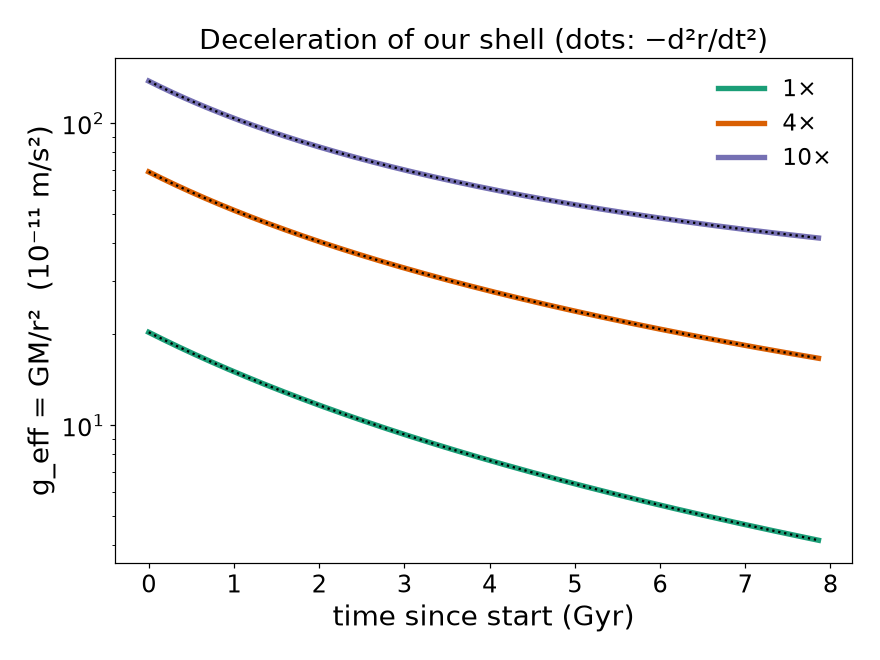
\includegraphics[width=0.48\textwidth]{p1_geff.png}\hfill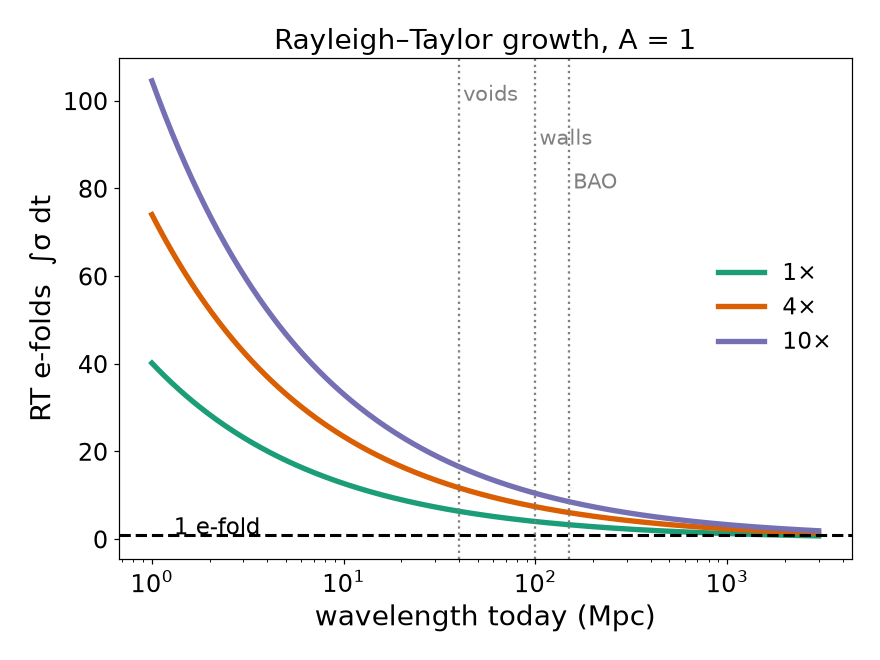
\includegraphics[width=0.48\textwidth]{p2_efolds.png}\\[4pt]
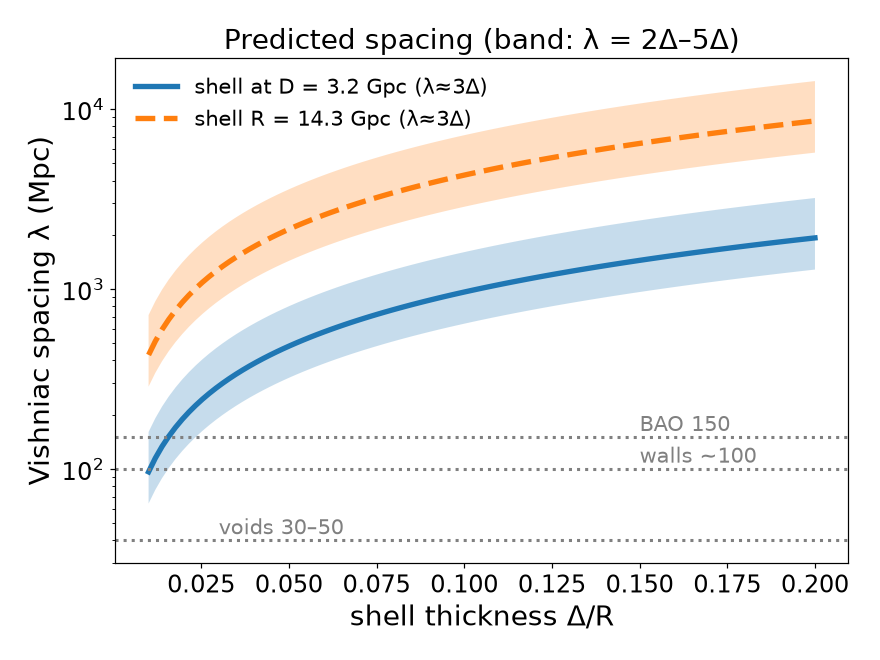
\includegraphics[width=0.48\textwidth]{p3_spacing.png}
\end{center}
\end{document}
